\documentclass[english]{article}
\usepackage{tikz}
\usepackage{pgfplots}
\pgfplotsset{compat=1.10}
\usetikzlibrary{shapes.geometric,arrows,fit,matrix,positioning}
\tikzset
{
    treenode/.style = {circle, draw=black, align=center, minimum size=1cm},
    subtree/.style  = {isosceles triangle, draw=black, align=center, minimum height=0.5cm, minimum width=1cm, shape border rotate=90, anchor=north}
}
\usepackage[letterpaper]{geometry}
\geometry{verbose,tmargin=1in,bmargin=1in,lmargin=1in,rmargin=1in}
\usepackage{babel}
\usepackage{amsmath}
\usepackage{amssymb}
\usepackage{capt-of}
\usepackage{graphicx}
\usepackage{color}
\usepackage{latexsym}
\usepackage{xspace}
\usepackage{pdflscape}
\usepackage[hyphens]{url}
\usepackage[colorlinks]{hyperref}
\usepackage{enumerate}
\usepackage{ifthen}
\usepackage{float}
\usepackage{array}
\usepackage{tikz}
\usepackage{multirow} 
\usetikzlibrary{shapes}
\usepackage{algorithm2e}
\usepackage{listings}

%%%% CUSTOM MATH GOES HERE
\newcommand{\ind}[1]{\mathbf{1}\left(#1\right)}
\renewcommand{\Pr}{\mathbf{Pr}\xspace}
\newcommand{\Bern}{\textsf{Bernoulli}\xspace}
\newcommand{\sign}{\textsf{sign}}
\newcommand{\E}{\mathbf{E}}
\newcommand{\bx}{\mathbf{x}}
\newcommand{\bX}{\mathbf{X}}
\newcommand{\by}{\mathbf{y}}
\newcommand{\bY}{\mathbf{Y}}
\newcommand{\bz}{\mathbf{z}}
\newcommand{\bw}{\mathbf{w}}
\newcommand{\bl}{\mathbf{\ell}}
\newcommand{\vc}[1]{\mathbf{#1}}
\newcommand{\Hypo}{\mathcal{H}}
\newcommand{\XX}{\mathcal{X}}
\newcommand{\cD}{\mathcal{D}}
\newcommand{\argmax}{\operatornamewithlimits{argmax}}
\newcommand{\argmin}{\operatornamewithlimits{argmin}}
\newcolumntype{M}{>{$\vcenter\bgroup\hbox\bgroup}c<{\egroup\egroup$}}
\newcolumntype{x}[1]{>{\centering\arraybackslash}m{#1}}

%%%%%%%%%%%%%%%%%%%%%%%%%%%%%%%%%
\title{CIS 520, Machine Learning, Fall 2018: Assignment 4\\}
\date{}
\author{Wentao He}

\begin{document}
\maketitle
{\normalsize Collaborator: \underline{N/A}}


\section{Convolutional Neural Network}
\begin{enumerate}
    \item Number of weights = $108 \times 163 \times 3 = \boxed{52488}$
    
    \item Number of weights = $18 \times 6 \times 3 = \boxed{324}$
    
    \item Number of neurons = $\dfrac{108-18}{6}+1 = \boxed{16}$ and $\dfrac{162-6}{6}+1 = \boxed{27}$ in $x$ and $y$ directions respectively. So the total number of neurons is $16 \times 27 = \boxed{432}$.
    
    \item \begin{equation*}
  \text{output filter 1} = \boxed{
    \begin{bmatrix}
    8&9&10\\
    11&-5&13\\
    2&3&11\\
    \end{bmatrix}} \quad\quad
  \text{output filter 2} = \boxed{
    \begin{bmatrix}
    2&17&0\\
    26&-13&16\\
    9&16&-5\\
    \end{bmatrix}}
\end{equation*}
\end{enumerate}
\clearpage


\section{Optimization and Lagrangian Duality}
\label{sec:optimization}

\begin{enumerate}
	\item 
	${\mathcal{L}}(x_1,x_2,\nu) = \boxed{\dfrac{1}{2}(x_1^2+x_2^2) + \nu(3x_1+2x_2-1)}$
	\item 
	$\dfrac{\partial \mathcal{L}}{\partial x_1} = x_1 + 3\nu = 0 \Rightarrow x_1 = -3\nu$\\\\
    $\dfrac{\partial \mathcal{L}}{\partial x_2} = x_2 + 2\nu = 0 \Rightarrow x_1 = -2\nu$\\\\
	$\therefore \phi(\nu) = \boxed{-\dfrac{13}{2}\nu^2-\nu}$
	\item 
	$\dfrac{\mathcal{L}}{dv} = -13\nu-1=0$\\\\
	$\nu^*= -\dfrac{1}{13}$\\\\
	$\therefore x_1^* = \boxed{\dfrac{3}{13}},  x_2^* =\boxed{\dfrac{2}{13}}$
\end{enumerate}
\clearpage

\section{Kernel Functions}

\begin{enumerate}
\item $\phi(x) = \boxed{\sqrt{c}\cdot K_2(x, x')}$
\item Such a mapping cannot exist (not a valid kernel) because for any given $c$, we cannot guarantee $K>0$.
\item $\phi(x) = \boxed{\left(\begin{array}{c}
      \phi_1(x) \\
      \phi_2(x)
    \end{array}\right)}$
\item $\phi(x) = \boxed{\left[\begin{array}{c}
      \phi_1(x) \\
      \phi_1(x) \\
      \vdots\\
      \phi_1(x)
    \end{array}\right] \circ \left[\begin{array}{c}
      \phi_{21}(x) \\
      \vdots\\
      \phi_{21}(x) \\
      \vdots\\
      \phi_{2d_2}(x)\\
      \vdots\\
      \phi_{2d_2}(x)
    \end{array}\right]}$\\
    The left vector consists of $d_2$ rows of $\phi_1$. The right vector consists of $d_1$ rows of $\phi_2$. $\circ$ is the element-wise multiplication between the two vectors.
\item $\phi(x) = \boxed{\phi_1(f(x))}$
\end{enumerate}
\clearpage



\section{SVM and Neural Nets: Programming Exercise}
\subsection{SVM on synthetic data}
\begin{enumerate}
\item
\begin{enumerate}
\item Cross Validation Error = \boxed{0.0840}
\item Training Error = \boxed{0.0860}
\item Test Error = \boxed{0.1090}\\\\
For the plot, please see Figure \ref{fig:411}.\\
        \begin{figure}[H]
          \centering
          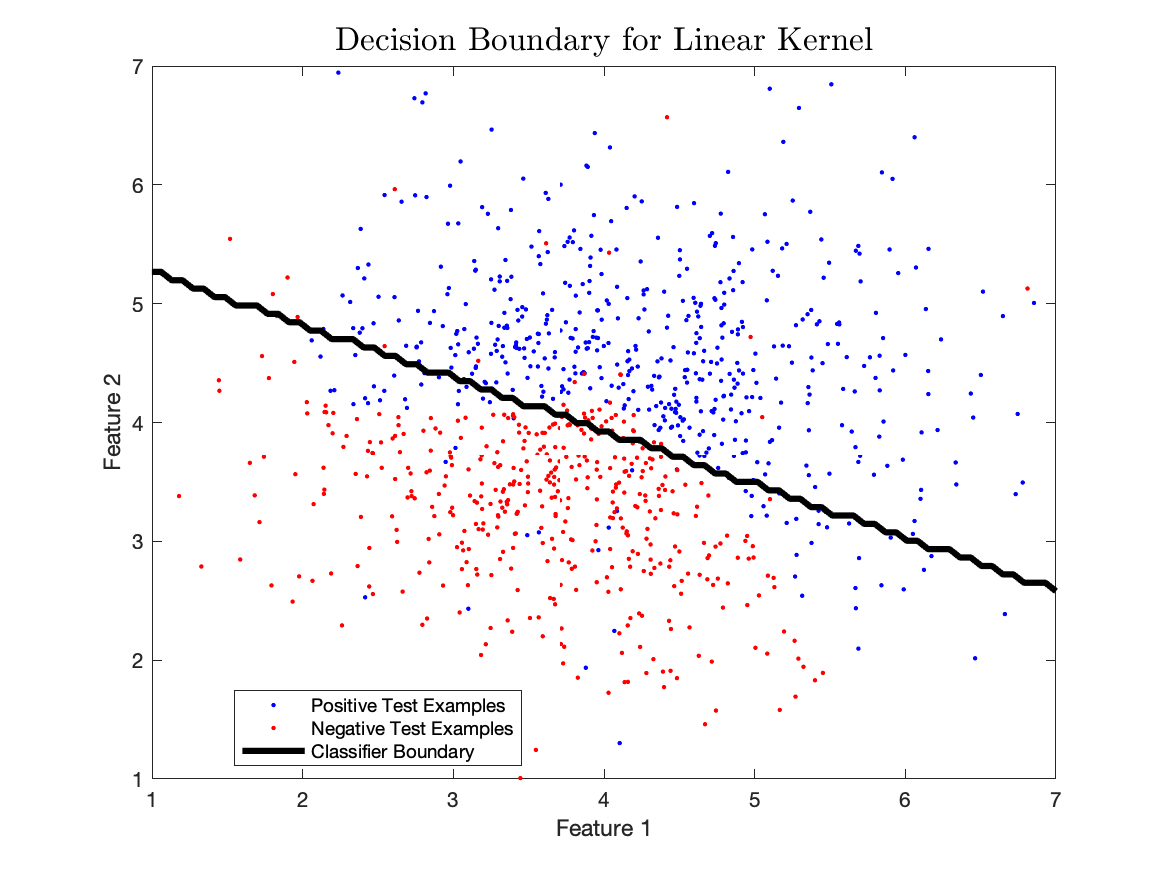
\includegraphics[width=0.7\textwidth]{LinearKernel.png}
          \caption{Decision Boundary for Linear Kernel.}
          \label{fig:411}
        \end{figure}
\end{enumerate}
\clearpage
\item 
\begin{enumerate}

\item When $\boxed{\sigma = 0.1, C = 0.1}$ For the plot, please see Figure \ref{fig:01}.\\
        \begin{figure}[H]
          \centering
          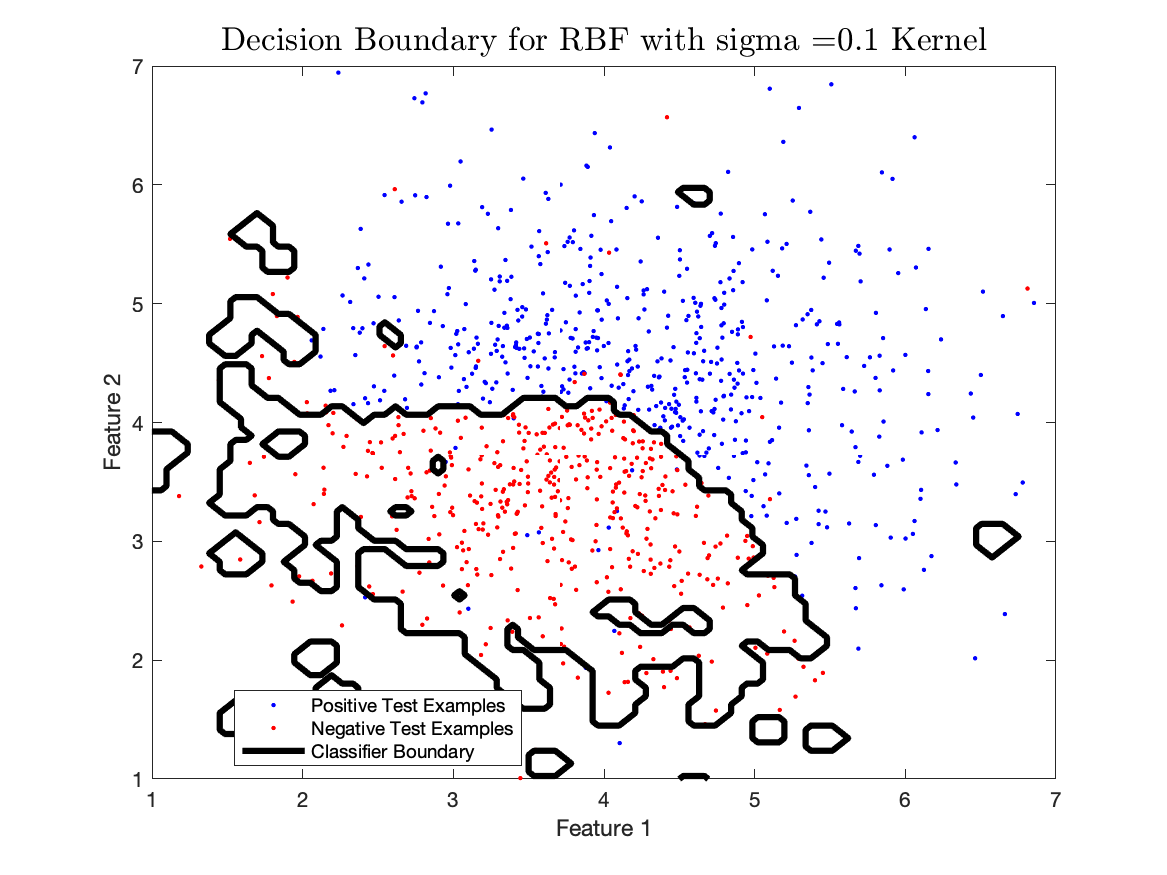
\includegraphics[width=0.7\textwidth]{01.png}
          \caption{Decision Boundary for RBF Kernel with $\sigma = 0.1$.}
          \label{fig:01}
        \end{figure}
\item When $\boxed{\sigma = 1, C = 100}$ For the plot, please see Figure \ref{fig:1}.\\
        \begin{figure}[H]
          \centering
          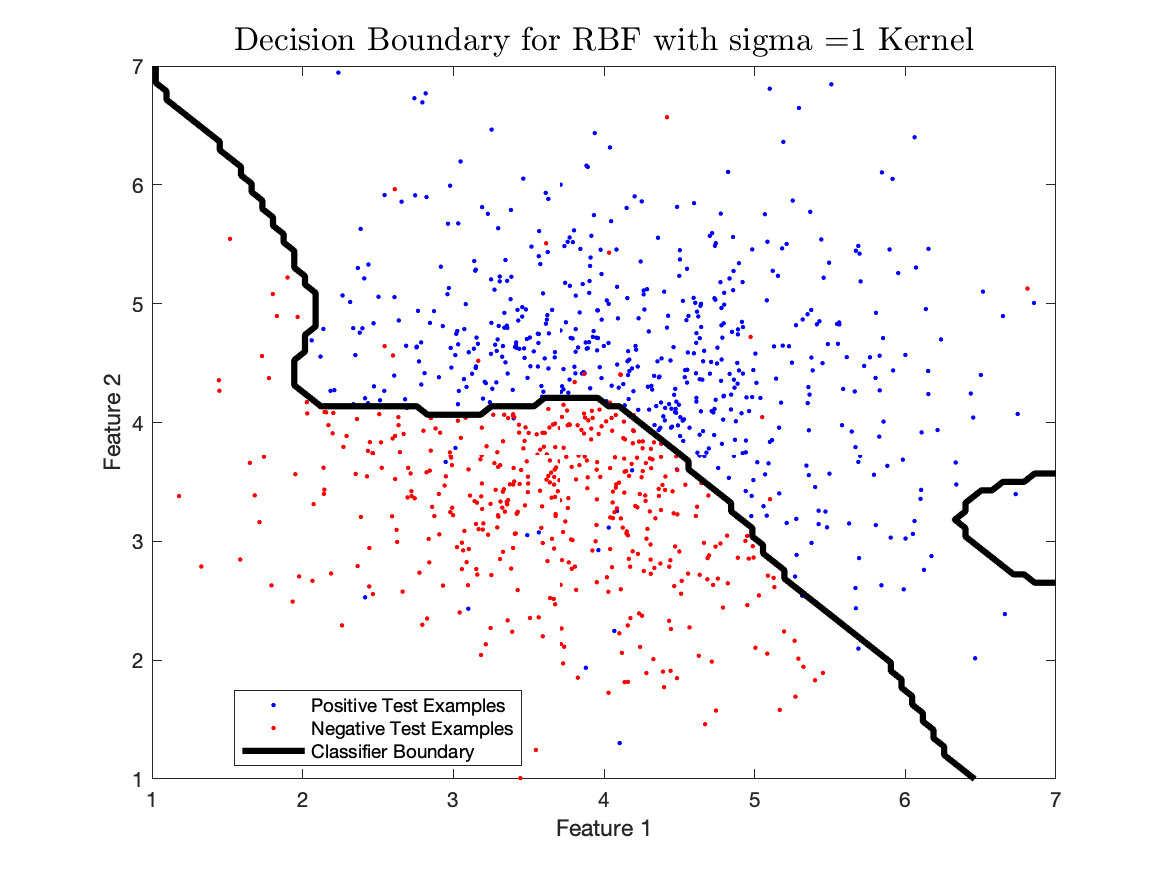
\includegraphics[width=0.7\textwidth]{1.png}
          \caption{Decision Boundary for RBF Kernel with $\sigma = 1$.}
          \label{fig:1}
        \end{figure}
        \clearpage
\item When $\boxed{\sigma = 10, C = 100000}$ For the plot, please see Figure \ref{fig:10}.\\
        \begin{figure}[H]
          \centering
          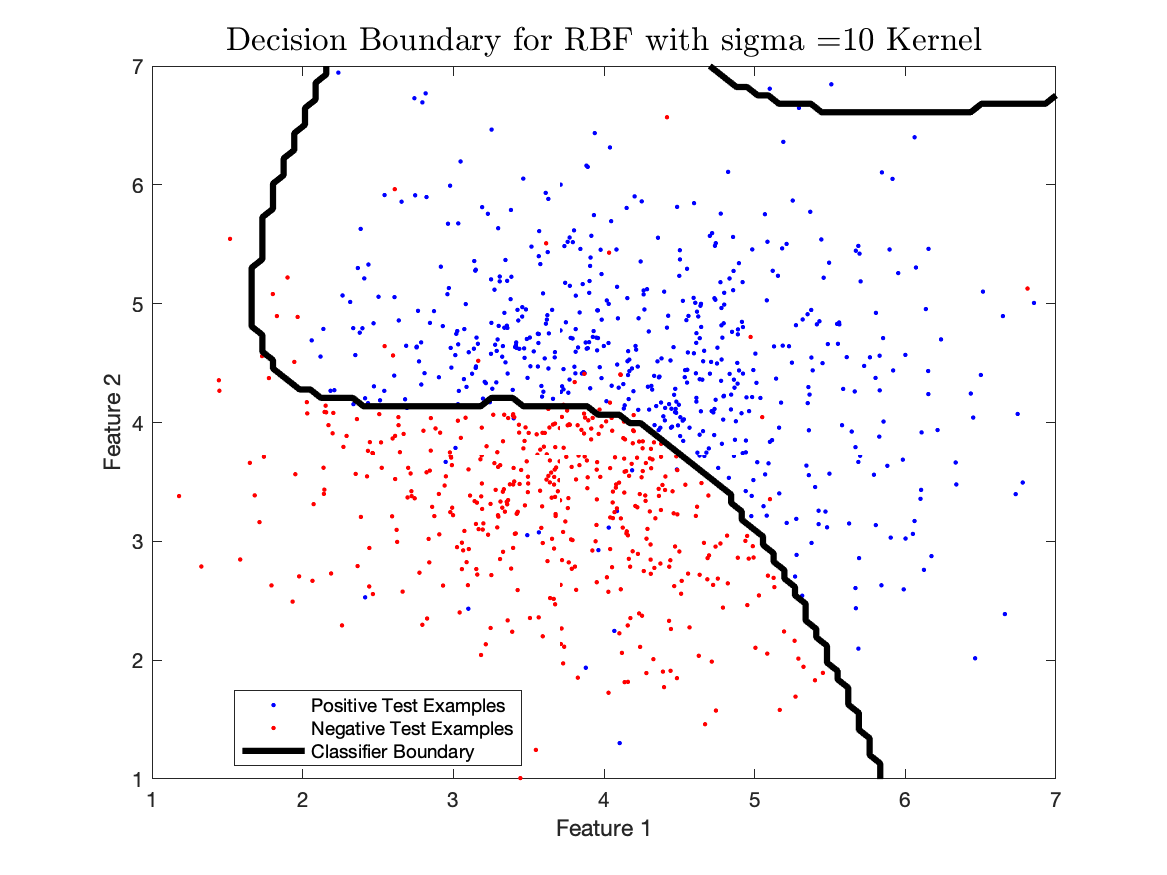
\includegraphics[width=0.7\textwidth]{10.png}
          \caption{Decision Boundary for RBF Kernel with $\sigma = 10$.}
          \label{fig:10}
        \end{figure}
\item When $\boxed{\sigma = 100, C = 100000}$ For the plot, please see Figure \ref{fig:100}.\\
        \begin{figure}[H]
          \centering
          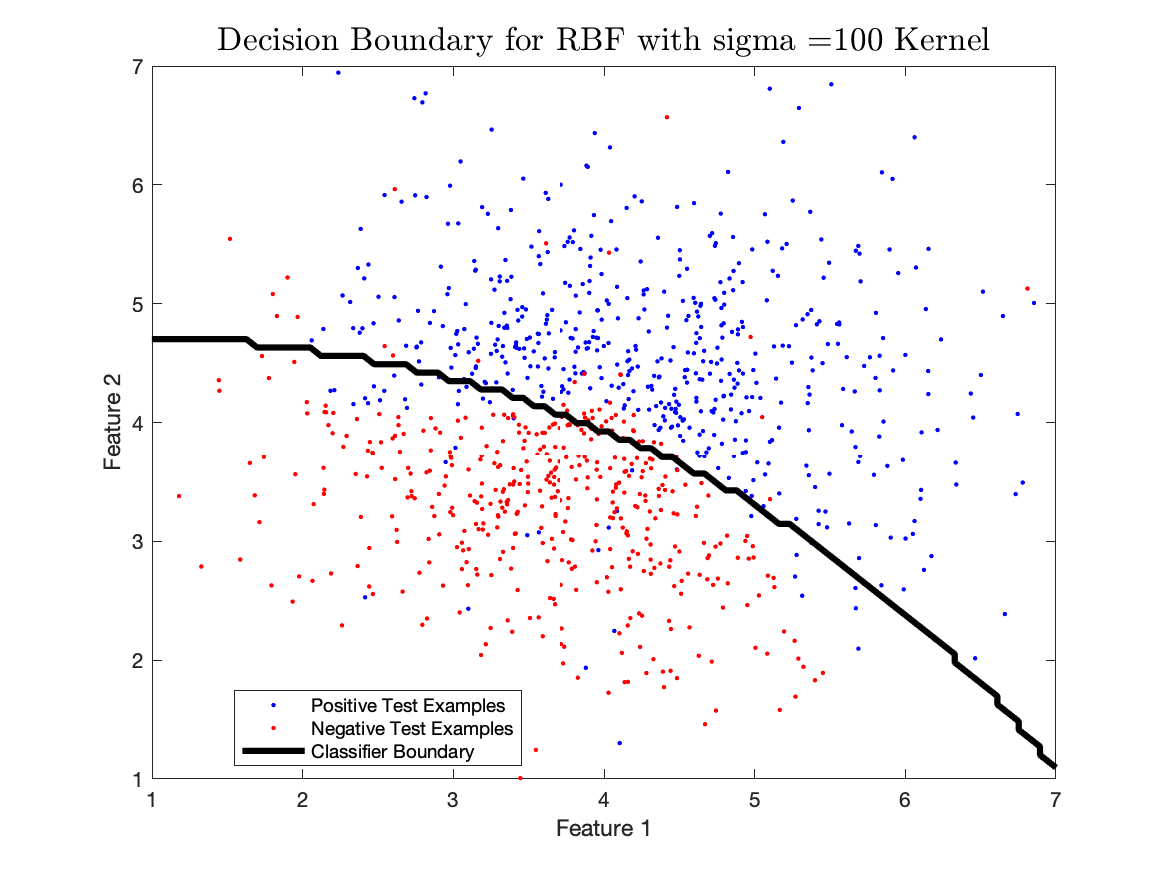
\includegraphics[width=0.7\textwidth]{100.png}
          \caption{Decision Boundary for RBF Kernel with $\sigma = 100$.}
          \label{fig:100}
        \end{figure}
        \clearpage
\item When $\boxed{\sigma = 1000, C = 100000}$ For the plot, please see Figure \ref{fig:1000}.\\
        \begin{figure}[H]
          \centering
          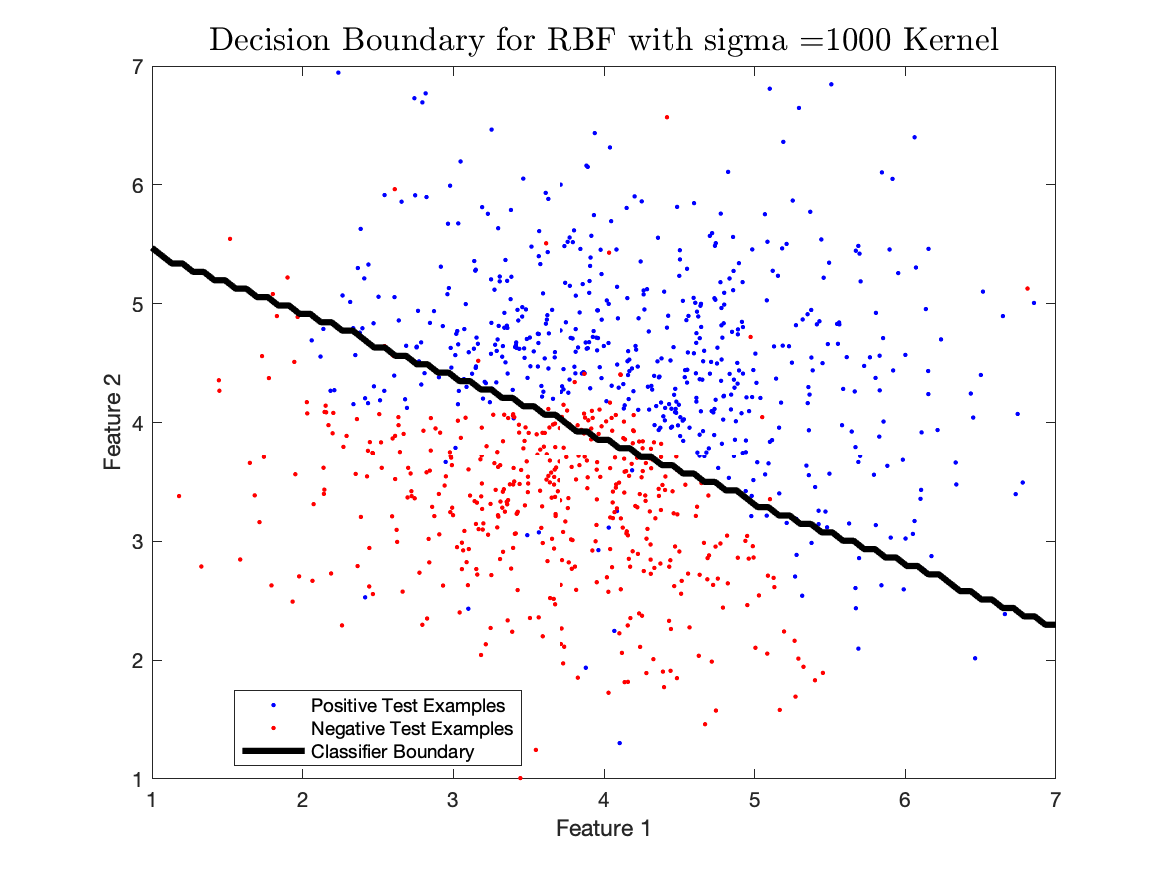
\includegraphics[width=0.7\textwidth]{1000.png}
          \caption{Decision Boundary for RBF Kernel with $\sigma = 1000$.}
          \label{fig:1000}
        \end{figure}

\item insert line plot of errors
For the plot, please see Figure \ref{fig:Error}.\\
        \begin{figure}[H]
          \centering
          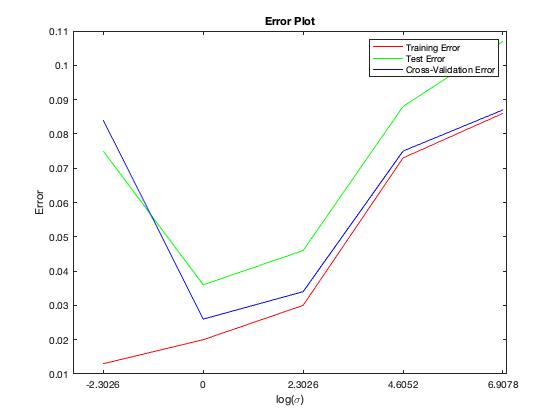
\includegraphics[width=0.7\textwidth]{ErrorPlot.png}
          \caption{Error Plot.}
          \label{fig:Error}
        \end{figure}
        \clearpage
\item $\sigma$ that achieves lowest test error is \boxed{1}.
\item $\sigma$ that achieves lowest cross-validation error is \boxed{1}.
\end{enumerate}
\item 
\begin{enumerate}
\item Absolute difference between test errors is \boxed{0.01}.
\item This difference in test errors is large. Selecting these parameters by cross-validation is a good approach because cross-validation error is very nearly unbiased for test error. The slight bias is due to that the training set in cross-validation is slightly smaller than the actual data set. In nearly all situations, the effect of this bias is conservative, i.e., the estimated fit is slightly biased in the direction suggesting a poorer fit. In practice, this bias is rarely a concern.
\end{enumerate}
\end{enumerate}
\subsection{SVM and Neural Nets on Breast Cancer Dataset}
\begin{enumerate}
    \item Summary of SVM results\\
    \begin{center}
      \begin{tabular}{|c |c |c |c| c|}
      \hline
      $\sigma$ & Best C & Train Error & Cross-Validation Error\\ [1ex]
      \hline
      0.1   &      1       &     0   &0.315\\[2ex]
      \hline
      1     &   10    &        0    &0.11667\\[2ex]
      \hline
      10   &      1    &    0.025     &0.03\\[2ex]
      \hline
      100     &   10  &   0.026667  &0.026667\\[2ex]
      \hline
      1000   &   1000  &   0.026667   &0.026667\\[2ex]
      \hline
      \end{tabular}
    \end{center}
    A table of $\sigma$, the best value of C, train error and cross-validation error are shown in the chart above. When $\sigma = 0.1$ and $\sigma = 1$, their train errors are equal to 0, and their cross-validation errors are high as well, which means over-fitting. When $\sigma = 100$ and $\sigma = 1000$, their cross-validation errors reach minimum and the SVM provides the best result.
    \item Summary of NN results
    \begin{center}
      \begin{tabular}{|c |c |c |c| c|}
      \hline
      & Best C & Train Error & Cross-Validation Error\\ [1ex]
      \hline
      ReLU + MSE  & 0.01&     0.0250       &     0.0283\\[2ex]
      \hline
      ReLU + Cross Entropy   &0 &   0.0433    &       0.0933\\[2ex]
      \hline
      Sigmoid + MSE   & 0&     0.0617    &    0.0433     \\[2ex]
      \hline
      Sigmoid + Cross Entropy &0.1    &   0.0417  &   0.0467\\[2ex]
      \hline
      \end{tabular}
    \end{center}
    A table of different combination of networks, best value of C, the corresponding train error and cross-validation error are shown in the chart above. However, each value is different after every round. However, generally speaking, MSE provides a better result than cross entropy due to its low cross-validation error. Based on the chart, ReLU + MSE gives the best result.
\end{enumerate}
\clearpage

\subsection{Appendix}
\textbf{Code for 4.2.1}
\color{red}
\begin{verbatim}
clc;
clear;

load('Breast-Cancer/trainingdata.mat');
load('Breast-Cancer/testdata.mat');

sigmas = [0.1,1,10,100,1000];
Boxconstrains = [1,10,100,1000,10000,100000];
Error = zeros(6,1);
train_err = zeros(5,1);
val_err = zeros(5,1);
Best_C = [];

for index = 1:size(sigmas, 2)
    sigma = sigmas(index)
    Error = zeros(6,1);
    for idx = 1:numel(Boxconstrains)
        err = 0;
        Boxconstrain = Boxconstrains(idx);
        for i = 1:5
            train_data = ['Breast-Cancer/CrossValidation/Fold',mat2str(i),'/cv-train.mat'];
            load(train_data);

            test_data = ['Breast-Cancer/CrossValidation/Fold',mat2str(i),'/cv-test.mat'];
            load(test_data);

            SVMModel = fitcsvm(cv_train(:,1:9),cv_train(:,10),'BoxConstraint',...
                Boxconstrain,'KernelFunction','rbf','KernelScale',sigma);

            labels= predict(SVMModel, cv_test(:,1:9));
            err = err + classification_error(labels, cv_test(:,10));
        end
        Error(idx,1) = err/5;
    end
    
    [Boxconstrains_min,column]=find(Error==min(min(Error)));
    if length(Boxconstrains_min) > 1
        Boxconstrains_min = Boxconstrains_min(1);
        column = column(1);
    end
    
    C = Boxconstrains(Boxconstrains_min)
    Best_C(end+1) = C;
    
    SVMModel = fitcsvm(train_inputs,train_labels,'BoxConstraint',...
        Boxconstrains(Boxconstrains_min),'KernelFunction','RBF','KernelScale',sigma);

    train_err(index,1) = classification_error(predict(SVMModel, train_inputs), train_labels)
    val_err(index,1) = Error(Boxconstrains_min,column)
    
end   
sigmas = sigmas';
Best_C = Best_C';
table(sigmas, Best_C, train_err, val_err)
  
SVMModel = fitcsvm(train_inputs,train_labels,'BoxConstraint',10,'KernelFunction','RBF',...
    'KernelScale',100);
labels = predict(SVMModel, test_inputs);
labels = sign(labels);
save('SVMlabels.mat','labels');
  
\end{verbatim}

\color{black}

\noindent\textbf{Code for 4.2.2}
\color{red}

\begin{verbatim}
clc;
clear;

load('Breast-Cancer/trainingdata.mat');
load('Breast-Cancer/testdata.mat');

Cs = [0,0.0001,0.001,0.01,0.1,1];
Cs_Err = zeros(6,1);

for index = 1:size(Cs, 2)        
    C = Cs(index);
    net = feedforwardnet([10]);
    net.layers{1}.transferFcn = 'poslin';
    %net.layers{1}.transferFcn = 'logsig';
    net.performFcn = 'crossentropy';
    %net.performFcn = 'mse';
    net.performParam.regularization = C;
    net.trainFcn = 'trainrp';
    
    err = 0;
    for i = 1:5
        train_data = ['Breast-Cancer/CrossValidation/Fold',mat2str(i),'/cv-train.mat'];
        load(train_data);

        test_data = ['Breast-Cancer/CrossValidation/Fold',mat2str(i),'/cv-test.mat'];
        load(test_data);

        net = train(net,cv_train(:,1:9)',cv_train(:,10)');
        labels= net(cv_test(:,1:9)');

        err = err + classification_error(sign(labels), cv_test(:,10)');
    end
    Cs_Err(index,1) = err/5;
    
end

[Cs_min,column]=find(Cs_Err==min(min(Cs_Err)));

if length(Cs_min) > 1
    Cs_min = Cs_min(1);
    column = column(1);
end

Best_c = Cs(Cs_min)
val_error = Cs_Err(Cs_min,column)

net = feedforwardnet(10);
net.layers{1}.transferFcn = 'poslin';
%net.layers{1}.transferFcn = 'logsig';
net.performFcn = 'crossentropy';
%net.performFcn = 'mse';
net.performParam.regularization = Cs(Cs_min);
net.trainFcn = 'trainrp';

net = train(net,train_inputs',train_labels');     
labels= net(test_inputs')';
labels = sign(labels);
save('NNlabels.mat','labels');

net = train(net,train_inputs',train_labels');     
labels= net(train_inputs')';
labels = sign(labels);
train_error = classification_error(sign(labels), train_labels)

\end{verbatim}
\end{document}
